\documentclass[10pt]{beamer}

\usepackage{settings}
\usepackage{minted}

\title{Cloud Computing}
\subtitle{Final Exam Exercise}
\date{\today}
\author[longname]{Giovanni Lucarelli}
\titlegraphic{\hfill
\includegraphics[height=1.3cm]{images/logo100_orizzontale.pdf}}

% add graphics path
\graphicspath{{../assets},{./images}}

\begin{document}

\maketitle

\section{Introduction}

\begin{frame}{Goal}
  1. \textbf{Build} a cluster of virtual nodes as:
  \begin{itemize}
    \item Virtual Machines $\rightarrow$ \alert{VirtualBox}
    \item Containers $\rightarrow$ \alert{Docker}
  \end{itemize}
  2. \textbf{Assess} and \textbf{compare} the performance:
  \begin{itemize}
    \item CPU
    \item Memory
    \item Disk I/O
    \item Network
  \end{itemize}
\end{frame}

\begin{frame}{(Virtual) Hardware Specification}
  \begin{columns}
    \hspace{0.5cm}\column{0.5\textwidth}
    {\footnotesize\textbf{\underline{Host Machine:}}
    \begin{description}
      \item[CPU] Intel Core i7-8550U CPU @ 1.80GHz, \\4 Cores / 8 Threads
      \item[Memory] 8 GB
      \item[Disk] 256 GB SSD
      \item[OS] Ubuntu 24.04.2 LTS
    \end{description}

    \textbf{\underline{Cluster Nodes:}}
    \begin{description}
      \item[CPU] 2 Cores
      \item[Memory] 2048 MB
      \item[Disk] 20 GB
      \item[OS] Ubuntu 22.04.5 live server
    \end{description}}
    \column{0.5\textwidth}
    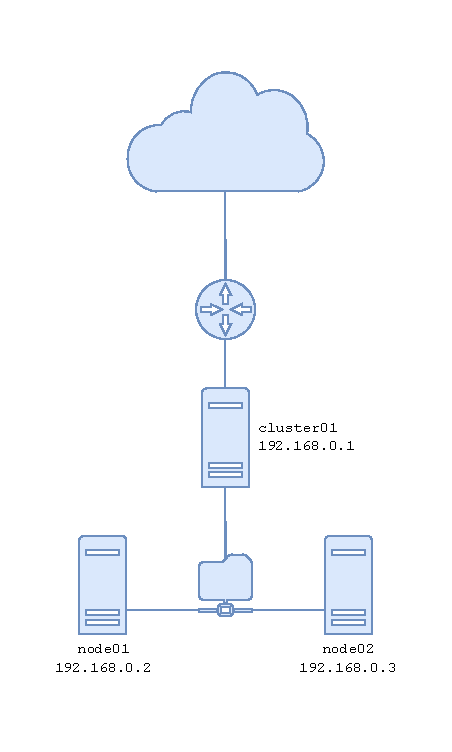
\includegraphics[width=0.9\linewidth]{images/diagram.pdf}
  \end{columns}
\end{frame}

\section{Methodology}
\begin{frame}{Virtual Machine Setup}
  \begin{enumerate}
    \item Build a template machine (hardware \& software) \& clone (reinitializing the MAC)
    \item Network Adapters (VirtualBox GUI):
    \begin{enumerate}
      \item NAT, internal net
      \item Port Forwarding and SSH (Host$\rightarrow$Master) 
    \end{enumerate}
    \item Master Node: 
    \begin{enumerate}
      \item \texttt{etc/hostname}, \texttt{etc/hosts}
      \item DHCP, DNS, gateway
      \item Shared file system (NFS)
    \end{enumerate}
    \item Worker Node: 
    \begin{enumerate}
      \item \texttt{etc/hostname}
      \item SSH (Master$\rightarrow$Worker)
      \item Shared file system (NFS)
    \end{enumerate}
  \end{enumerate}
  
\end{frame}


\begin{frame}[fragile]{Container Setup (1/2)}
\begin{enumerate}
\item Build a template machine (\alert{Dockerfile})
{\small\begin{verbatim}

# Download the latest official Ubuntu image
FROM ubuntu:latest

# Update and install all the required software
RUN apt-get update && apt-get install -y \ 
...
# Expose the SSH port
EXPOSE 22
\end{verbatim}}

\end{enumerate}
  
\end{frame}

\begin{frame}[fragile]{Container Setup (2/2)}
\begin{enumerate}
\setcounter{enumi}{1}
\item Build a cluster (\alert{Docker Compose})
\end{enumerate}
\begin{columns}
\column{0.2\textwidth}
{\footnotesize\begin{verbatim}
services:
  cluster01:
    ...
  node01:
    ...
  node02:
    ...    
networks:
  internal-net:
    driver: bridge
volumes:
  shared-data:
    driver: local
\end{verbatim}}
  \column{0.5\textwidth}
  {\footnotesize\begin{verbatim}
  cluster01:
    build: .
    container_name: cluster01
    hostname: cluster01
    networks:
      internal-net:  
    deploy:
      resources:
        limits:
          cpus: "2"
          memory: 2G
    ports:
      - "2220:22"
    volumes:
      - shared-data:/shared    
\end{verbatim}}

\end{columns}
  
\end{frame}

\begin{frame}{Benchmarks}
  \begin{description}
    \item[hpcc] suite of tests to measure the performance of high-performance computing systems
    \item[stress-ng] stress-testing CPUs, memory and other components under heavy load
    \item[sysbench] evaluating system parameters such as CPU, memory, and other components
    \item[iozone] measure filesystem I/O performance
    \item[iperf] measure network performance  
  \end{description}
\end{frame}

\begin{frame}{Assessing the Cluster}
  General guidelines:
  \begin{itemize}
    \item no heavy processes on the host during the tests
    \item repeat each test multiple times to account for variability ($1\leq n_i \leq 5$)
    \item monitorate the host resources during the tests
    \item repeat the tests on the host*
  \end{itemize}
  \end{frame}

\begin{frame}[fragile]{Running the tests}
  \begin{enumerate}
    \item \texttt{mpirun -np 4 -hostfile hosts <test>}\vspace{0.5cm}
 \\File \texttt{hosts}:
 \begin{verbatim}
 node01 slots=2
 node02 slots=2 
 \end{verbatim}
    \item bash-script to automatize multiple repetition of each test
  \end{enumerate}
 
\end{frame}

\section{Results}

\begin{frame}{High Performance Computing Challenge (HPCC)}
  Number of repetition: \textbf{3}

  Benchmark types:

\begin{itemize}

  \item \textbf{Computational}: HPL, DGEMM, FFT    
  \item \textbf{Memory}:   STREAM, PTRANS, RandomAccess
  \item \textbf{Communication}: PingPong, (PTRANS)

\end{itemize}

\end{frame}

\begin{frame}{HPCC: Computational Performance}
\begin{figure}
  \centering
  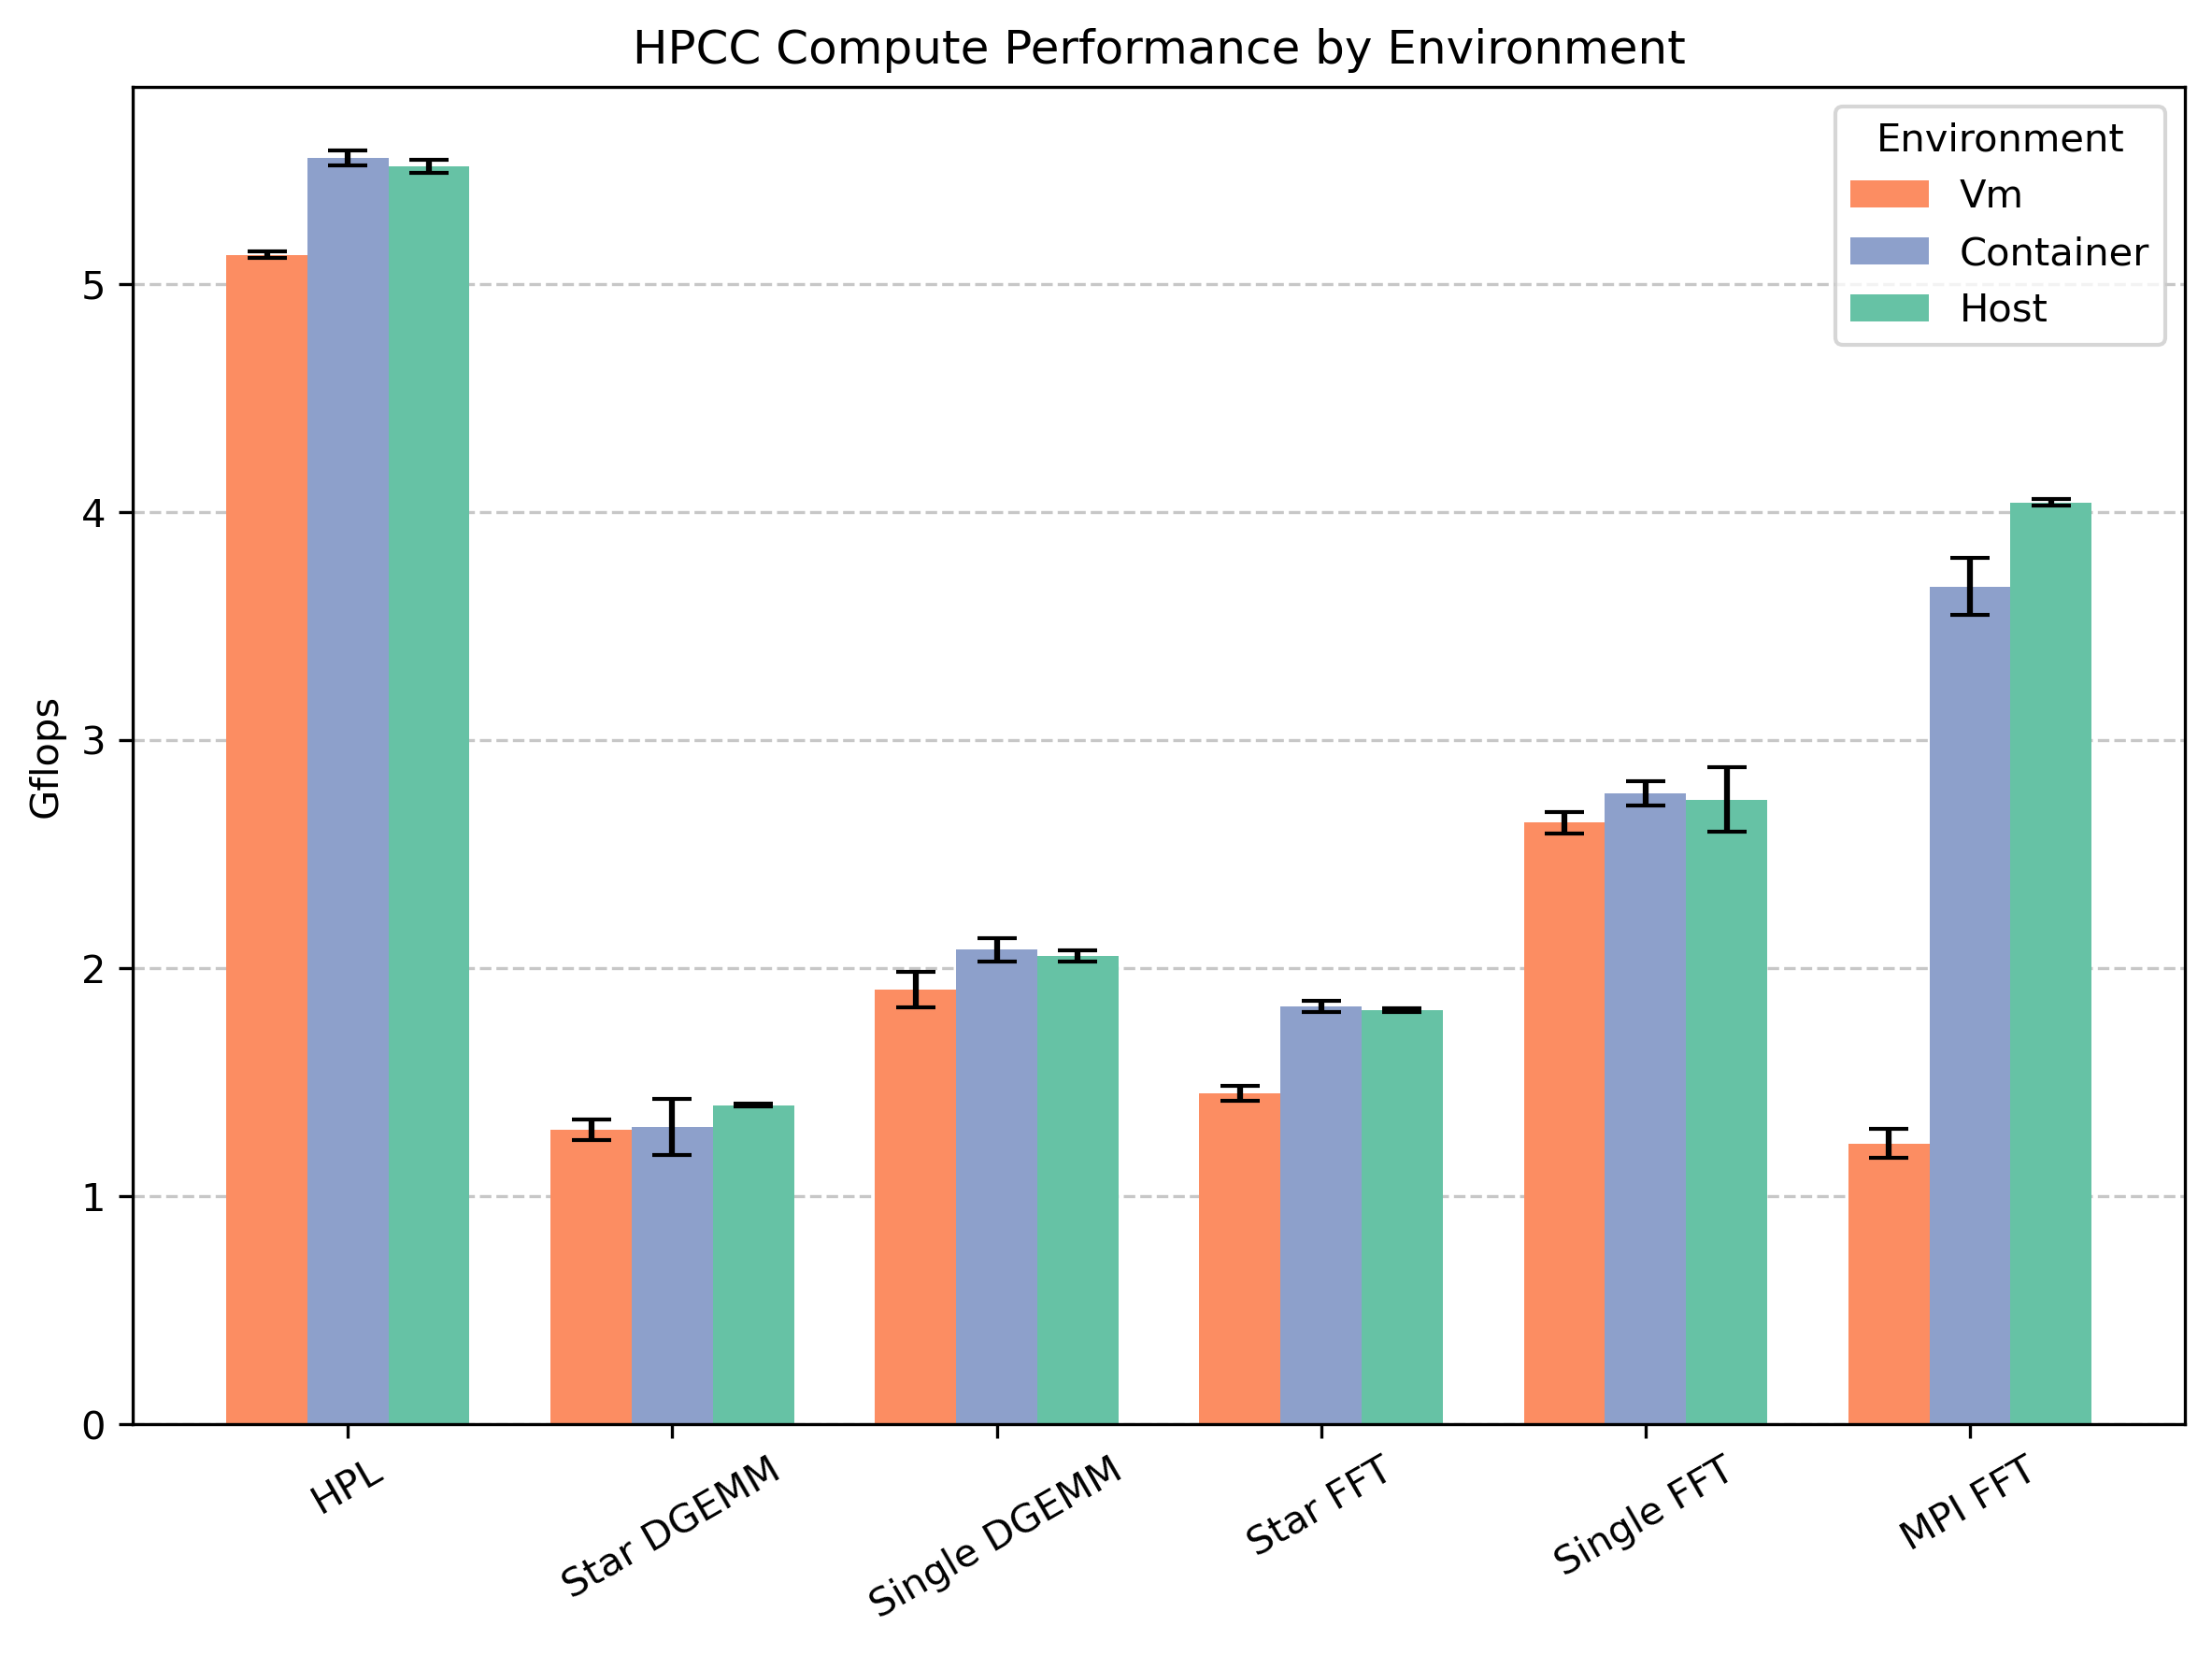
\includegraphics[width=0.8\textwidth]{hpcc_compute_performance.png}
\end{figure}

\end{frame}

\begin{frame}[fragile]{HPCC: Nominal Memory Bandwidth}
\texttt{sudo dmidecode --type memory}  
\begin{verbatim}
Configured Memory Speed: 1867 MT/s
Bus width per channel: 64 bits = 8 bytes
Number of channels: 2
\end{verbatim}
$$
\text{Bandwidth}\, \left[\frac{\text{GB}}{\text{s}}\right] = \text{2}\, \text{C} \times 1.867\, \text{GT} \times 8\, \frac{\text{B}}{\text{C}\,{T}} = 29.9\,\frac{\text{GB}}{\text{s}}
$$

\end{frame}

\begin{frame}{HPCC: Memory Performance (1/2)}
  \begin{table}[htbt]
  \centering
  \footnotesize
  \begin{tabular}{lccc}
  \toprule
  \textbf{Benchmark} & \textbf{VM} & \textbf{Container} & \textbf{Host} \\
  \midrule
  \textbf{SingleSTREAM (GB/s)} & & & \\
  Copy   & 22.30 ± 0.32 & $\mathbf{24.11 \pm 0.20}$ & 23.44 ± 0.06 \\
  Scale  & 13.26 ± 0.19 & 14.23 ± 0.06 & 14.06 ± 0.12 \\
  Add    & 14.40 ± 0.24 & 15.38 ± 0.16 & 15.06 ± 0.14 \\
  Triad  & 14.44 ± 0.28 & 15.48 ± 0.13 & 15.22 ± 0.05 \\
  \midrule
  \textbf{StarSTREAM (GB/s)} & & & \\
  Copy   & 5.03 ± 0.03 & $\mathbf{5.41 \pm 0.03}$ & 5.39 ± 0.02 \\
  Scale  & 3.34 ± 0.03 & 3.55 ± 0.01 & 3.56 ± 0.01 \\
  Add    & 3.75 ± 0.01 & 4.08 ± 0.02 & 4.07 ± 0.01 \\
  Triad  & 3.72 ± 0.04 & 4.02 ± 0.02 & 4.00 ± 0.02 \\
  \midrule
  \textbf{PTRANS (GB/s)} & $0.196 \pm 0.014$ & 1.181 ± 0.239 & $\mathbf{1.495 \pm 0.019}$ \\
  \bottomrule
  \end{tabular}
  \end{table}

\end{frame}



\begin{frame}{HPCC: Memory Performance (2/2)}
  \begin{figure}
    \centering
    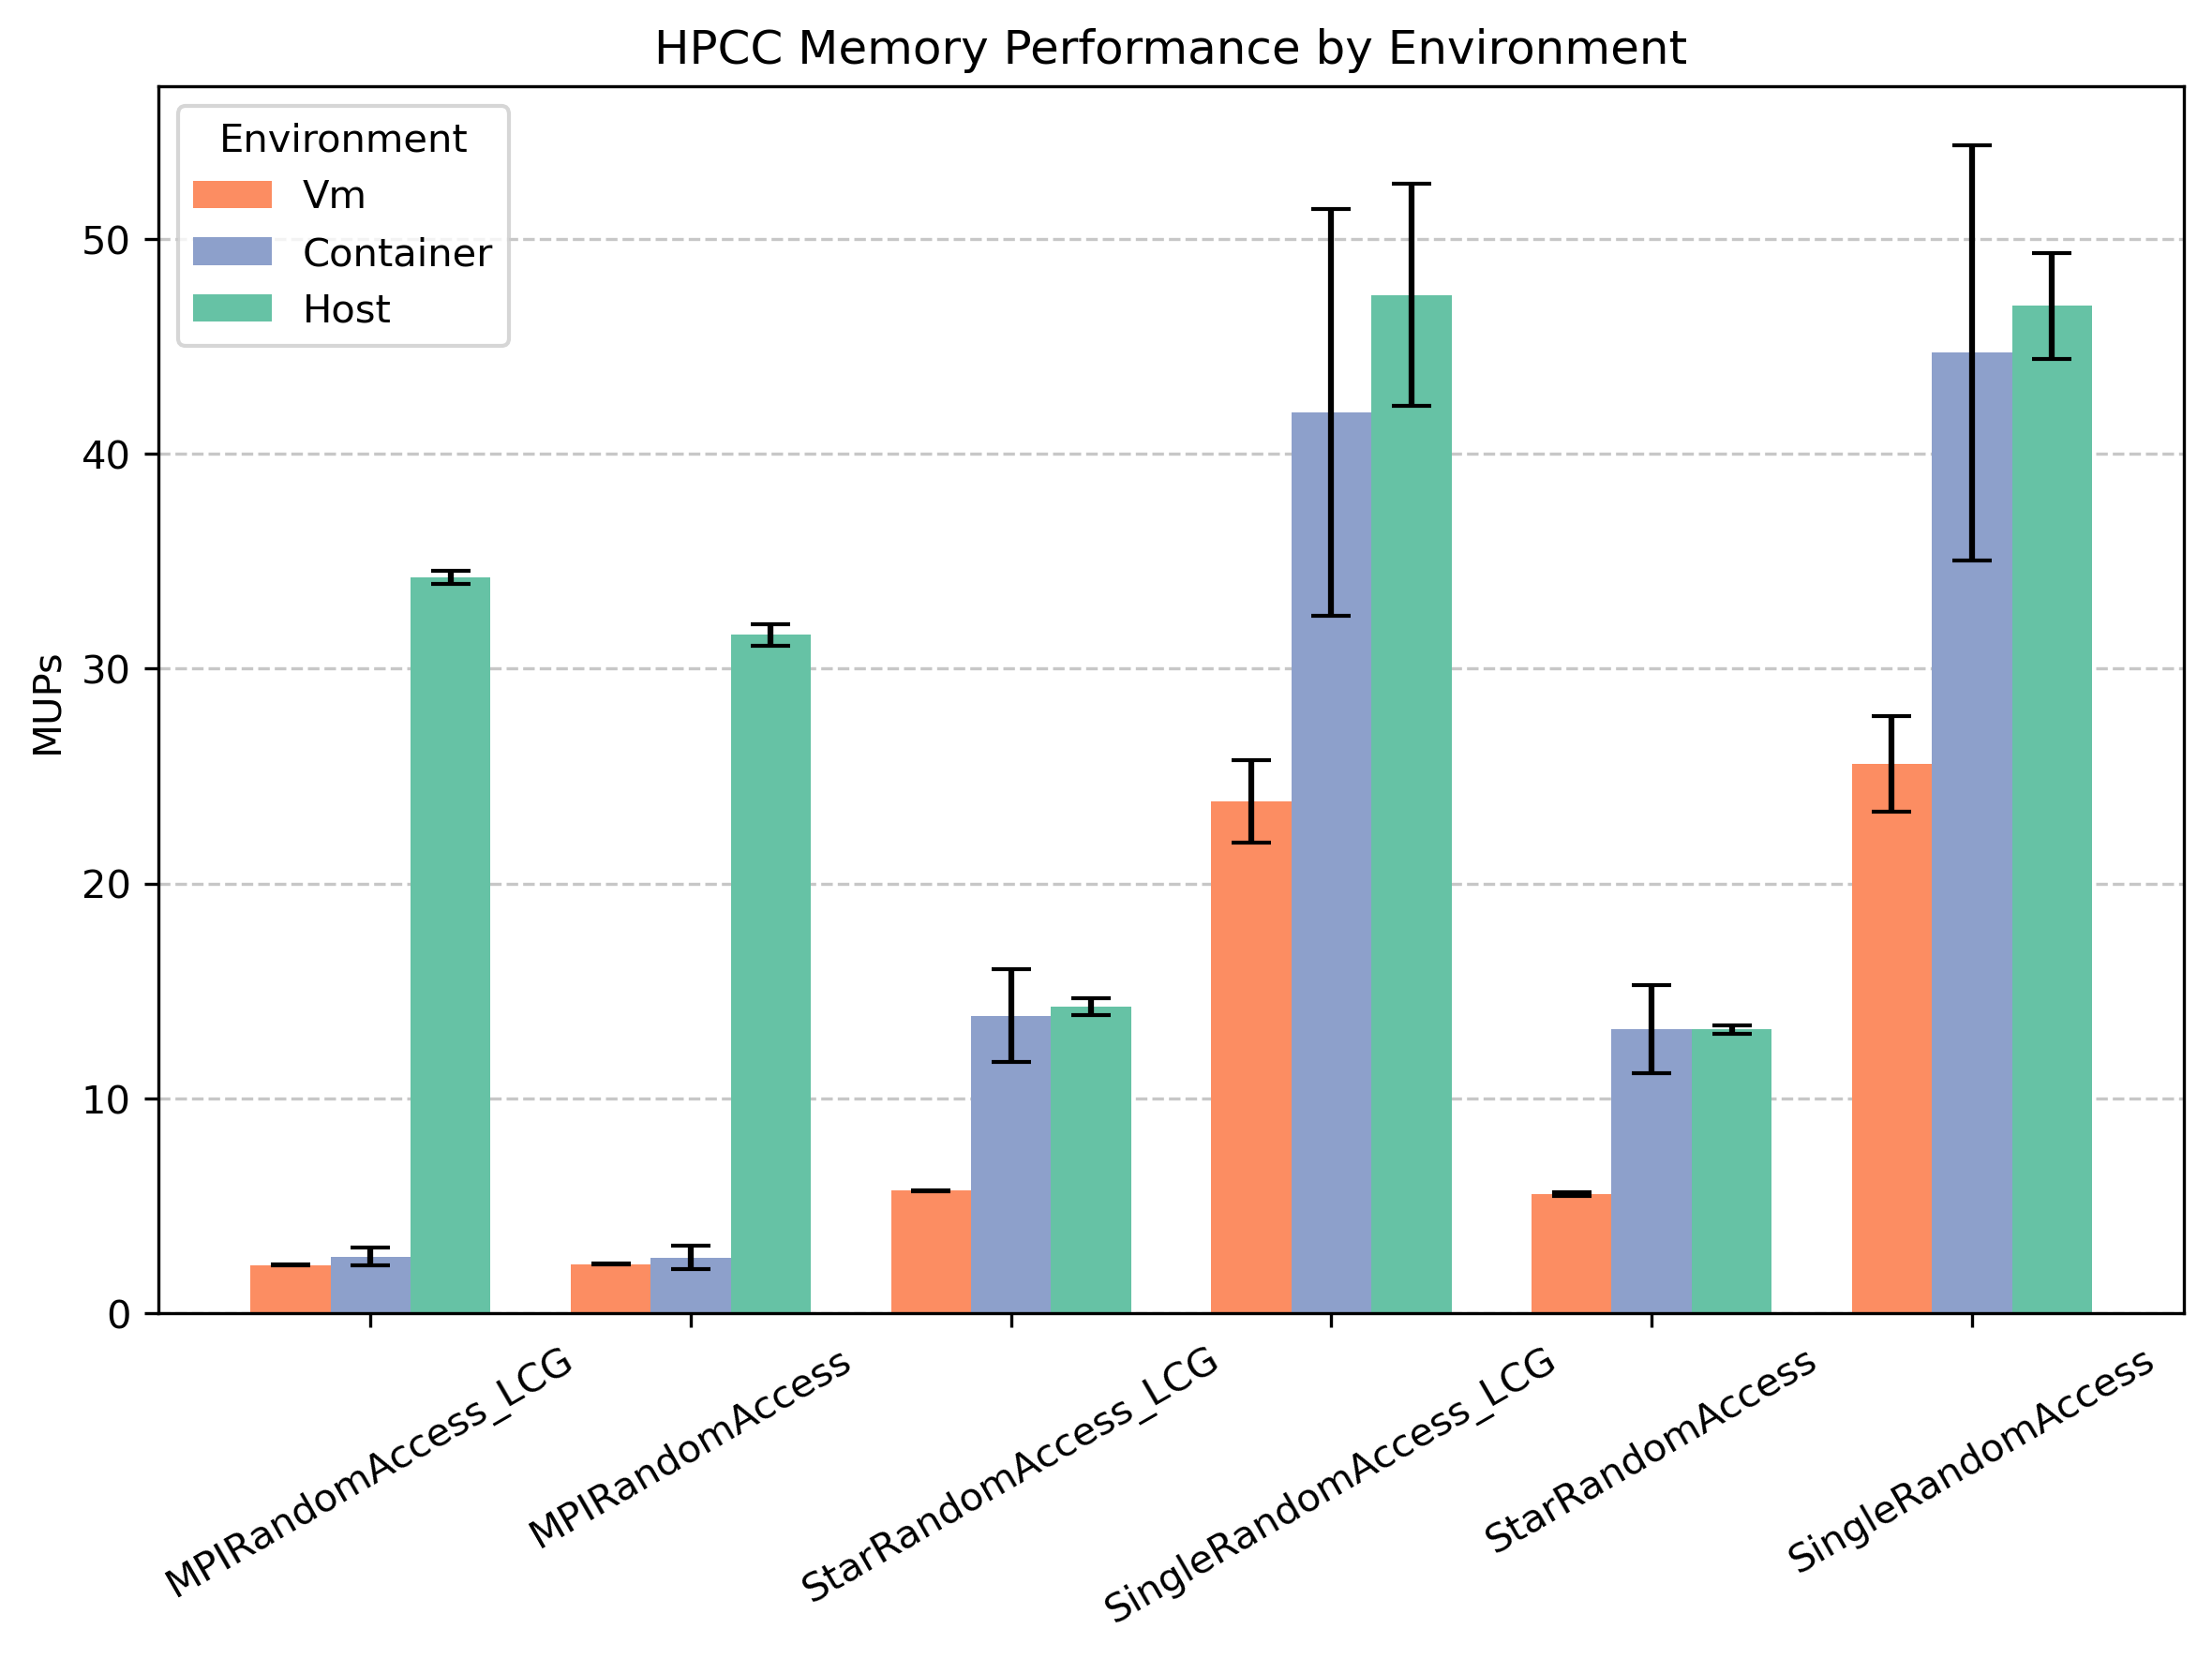
\includegraphics[width=0.8\textwidth]{hpcc_memory_performance.png}
  \end{figure}
\end{frame}

\begin{frame}{HPCC: Comunication Performance}
  \begin{figure}
    \centering
    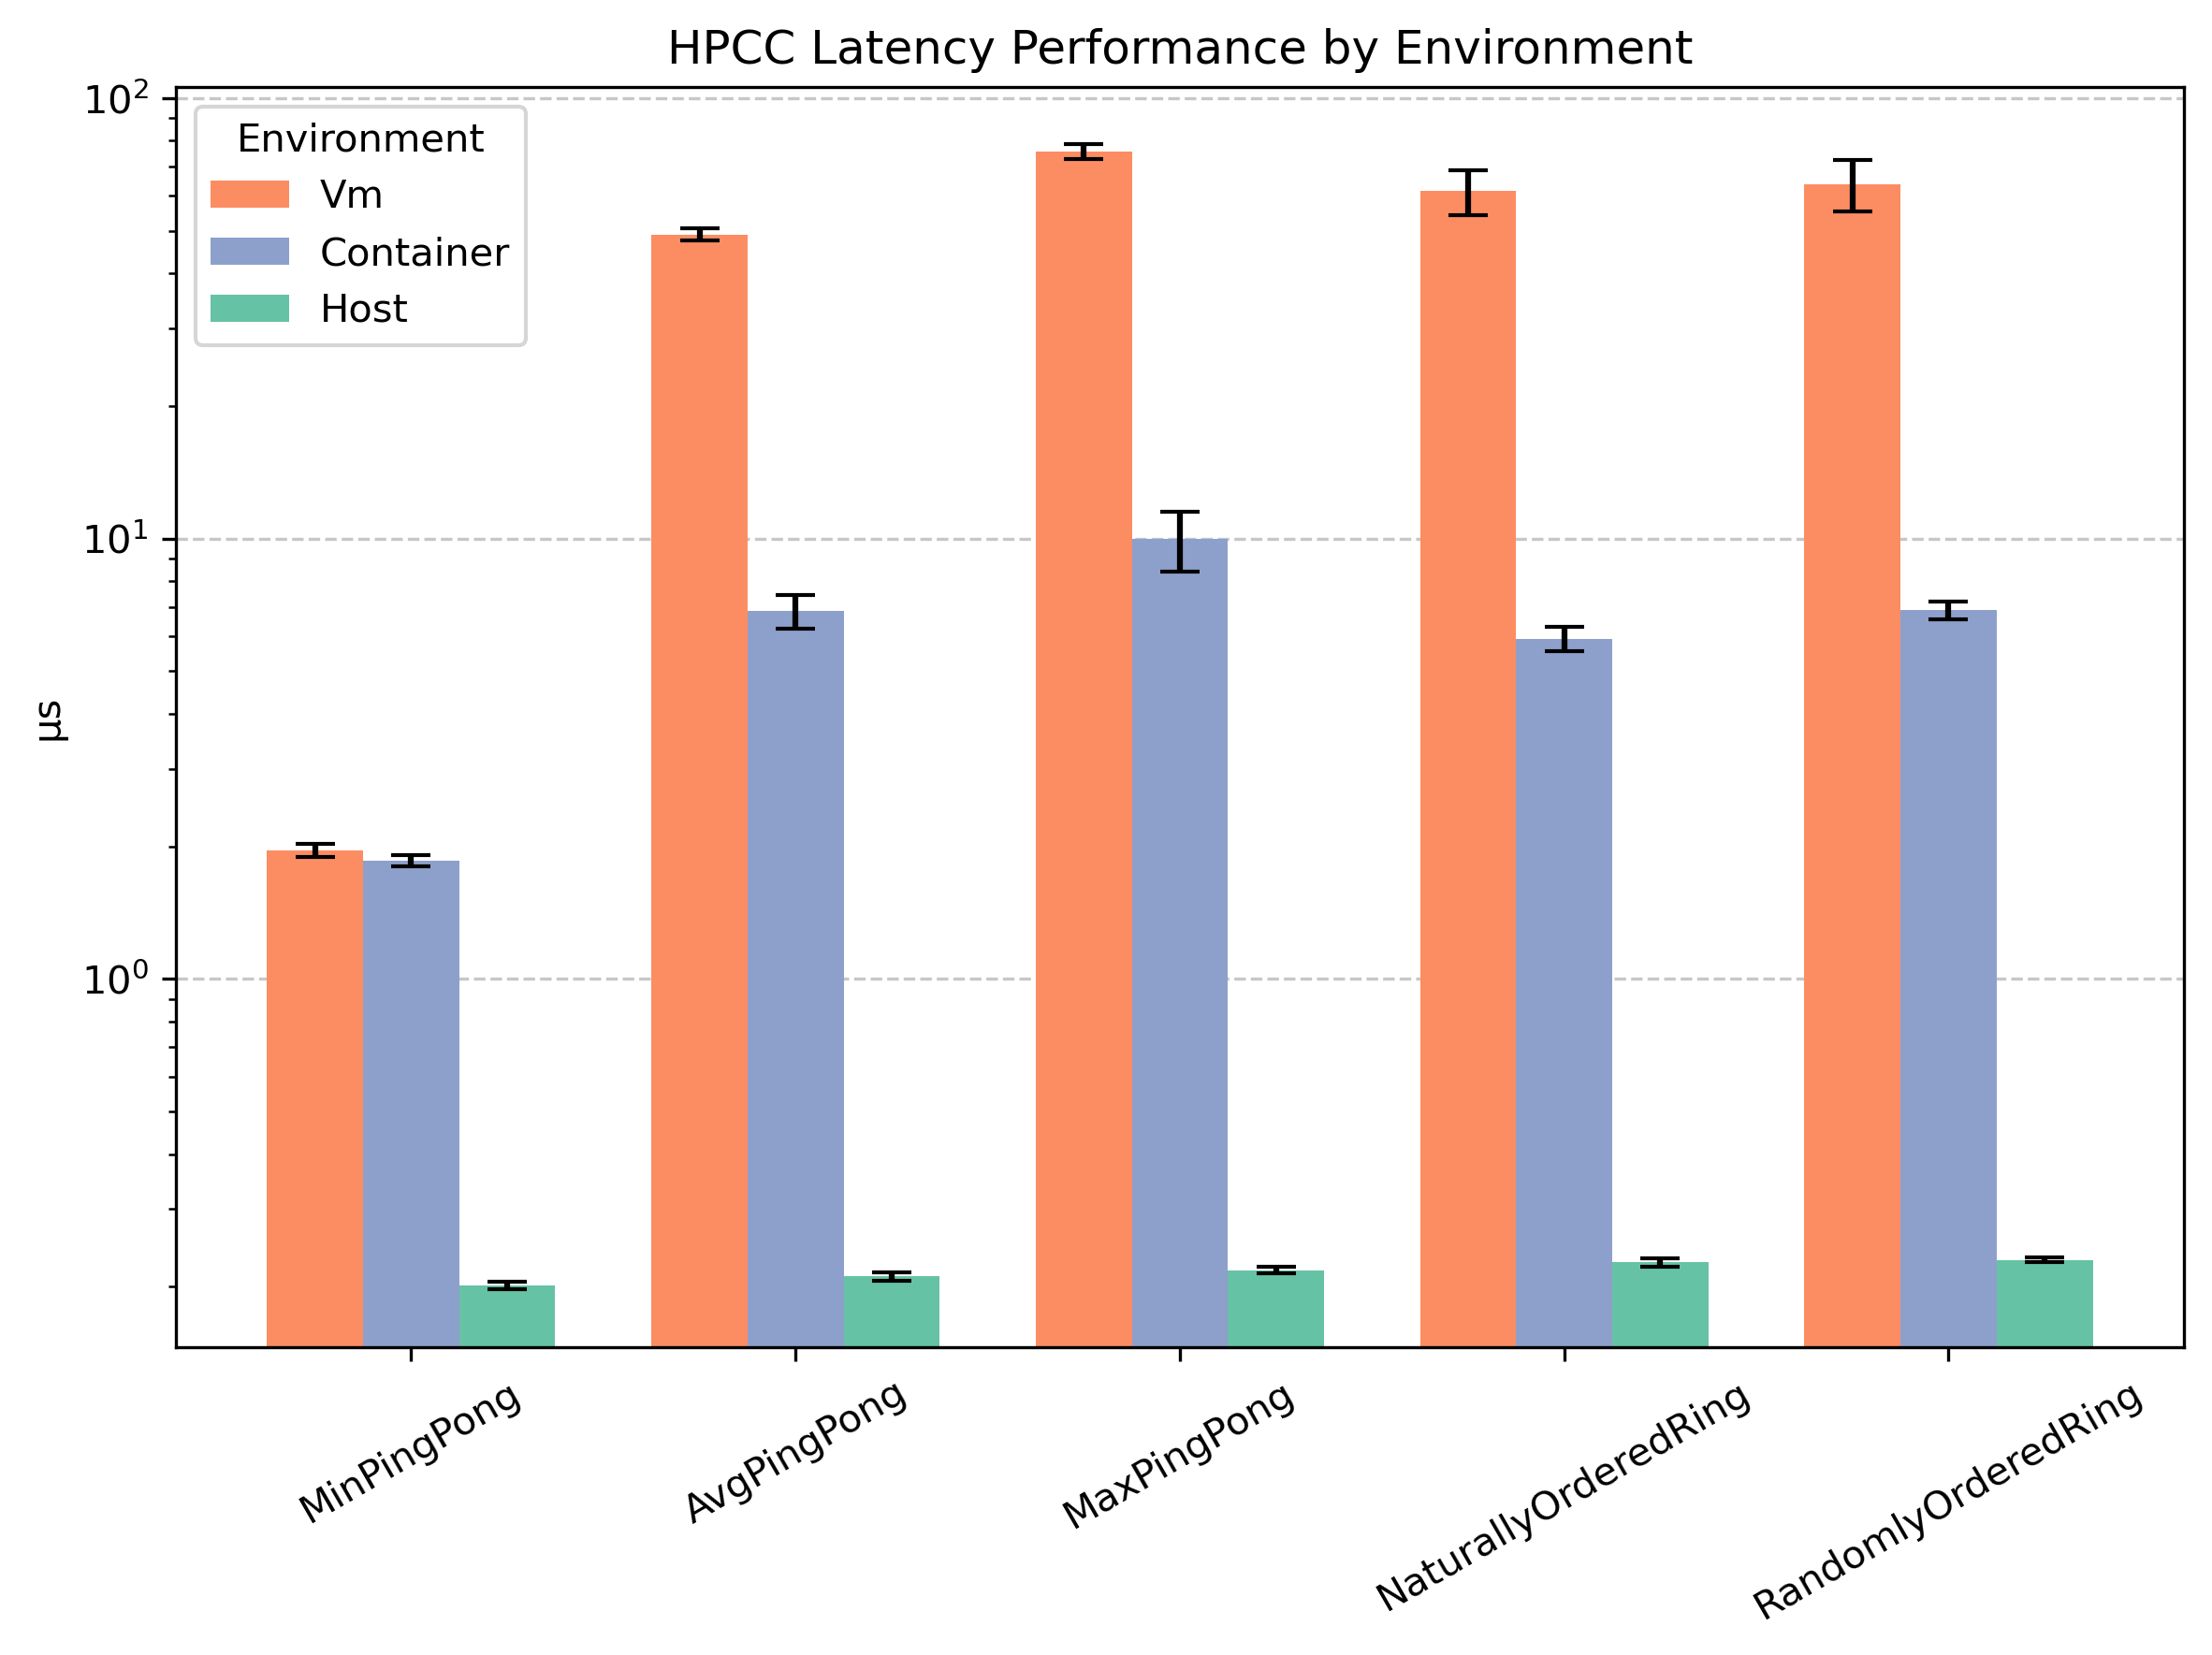
\includegraphics[width=0.8\textwidth]{hpcc_latency_performance.png}
  \end{figure}

  \centering{Note the \alert{log scale}!}
\end{frame}

\begin{frame}{Stress-ng: CPU}
  Repetitions: \textbf{5}
  \begin{figure}
    \centering
    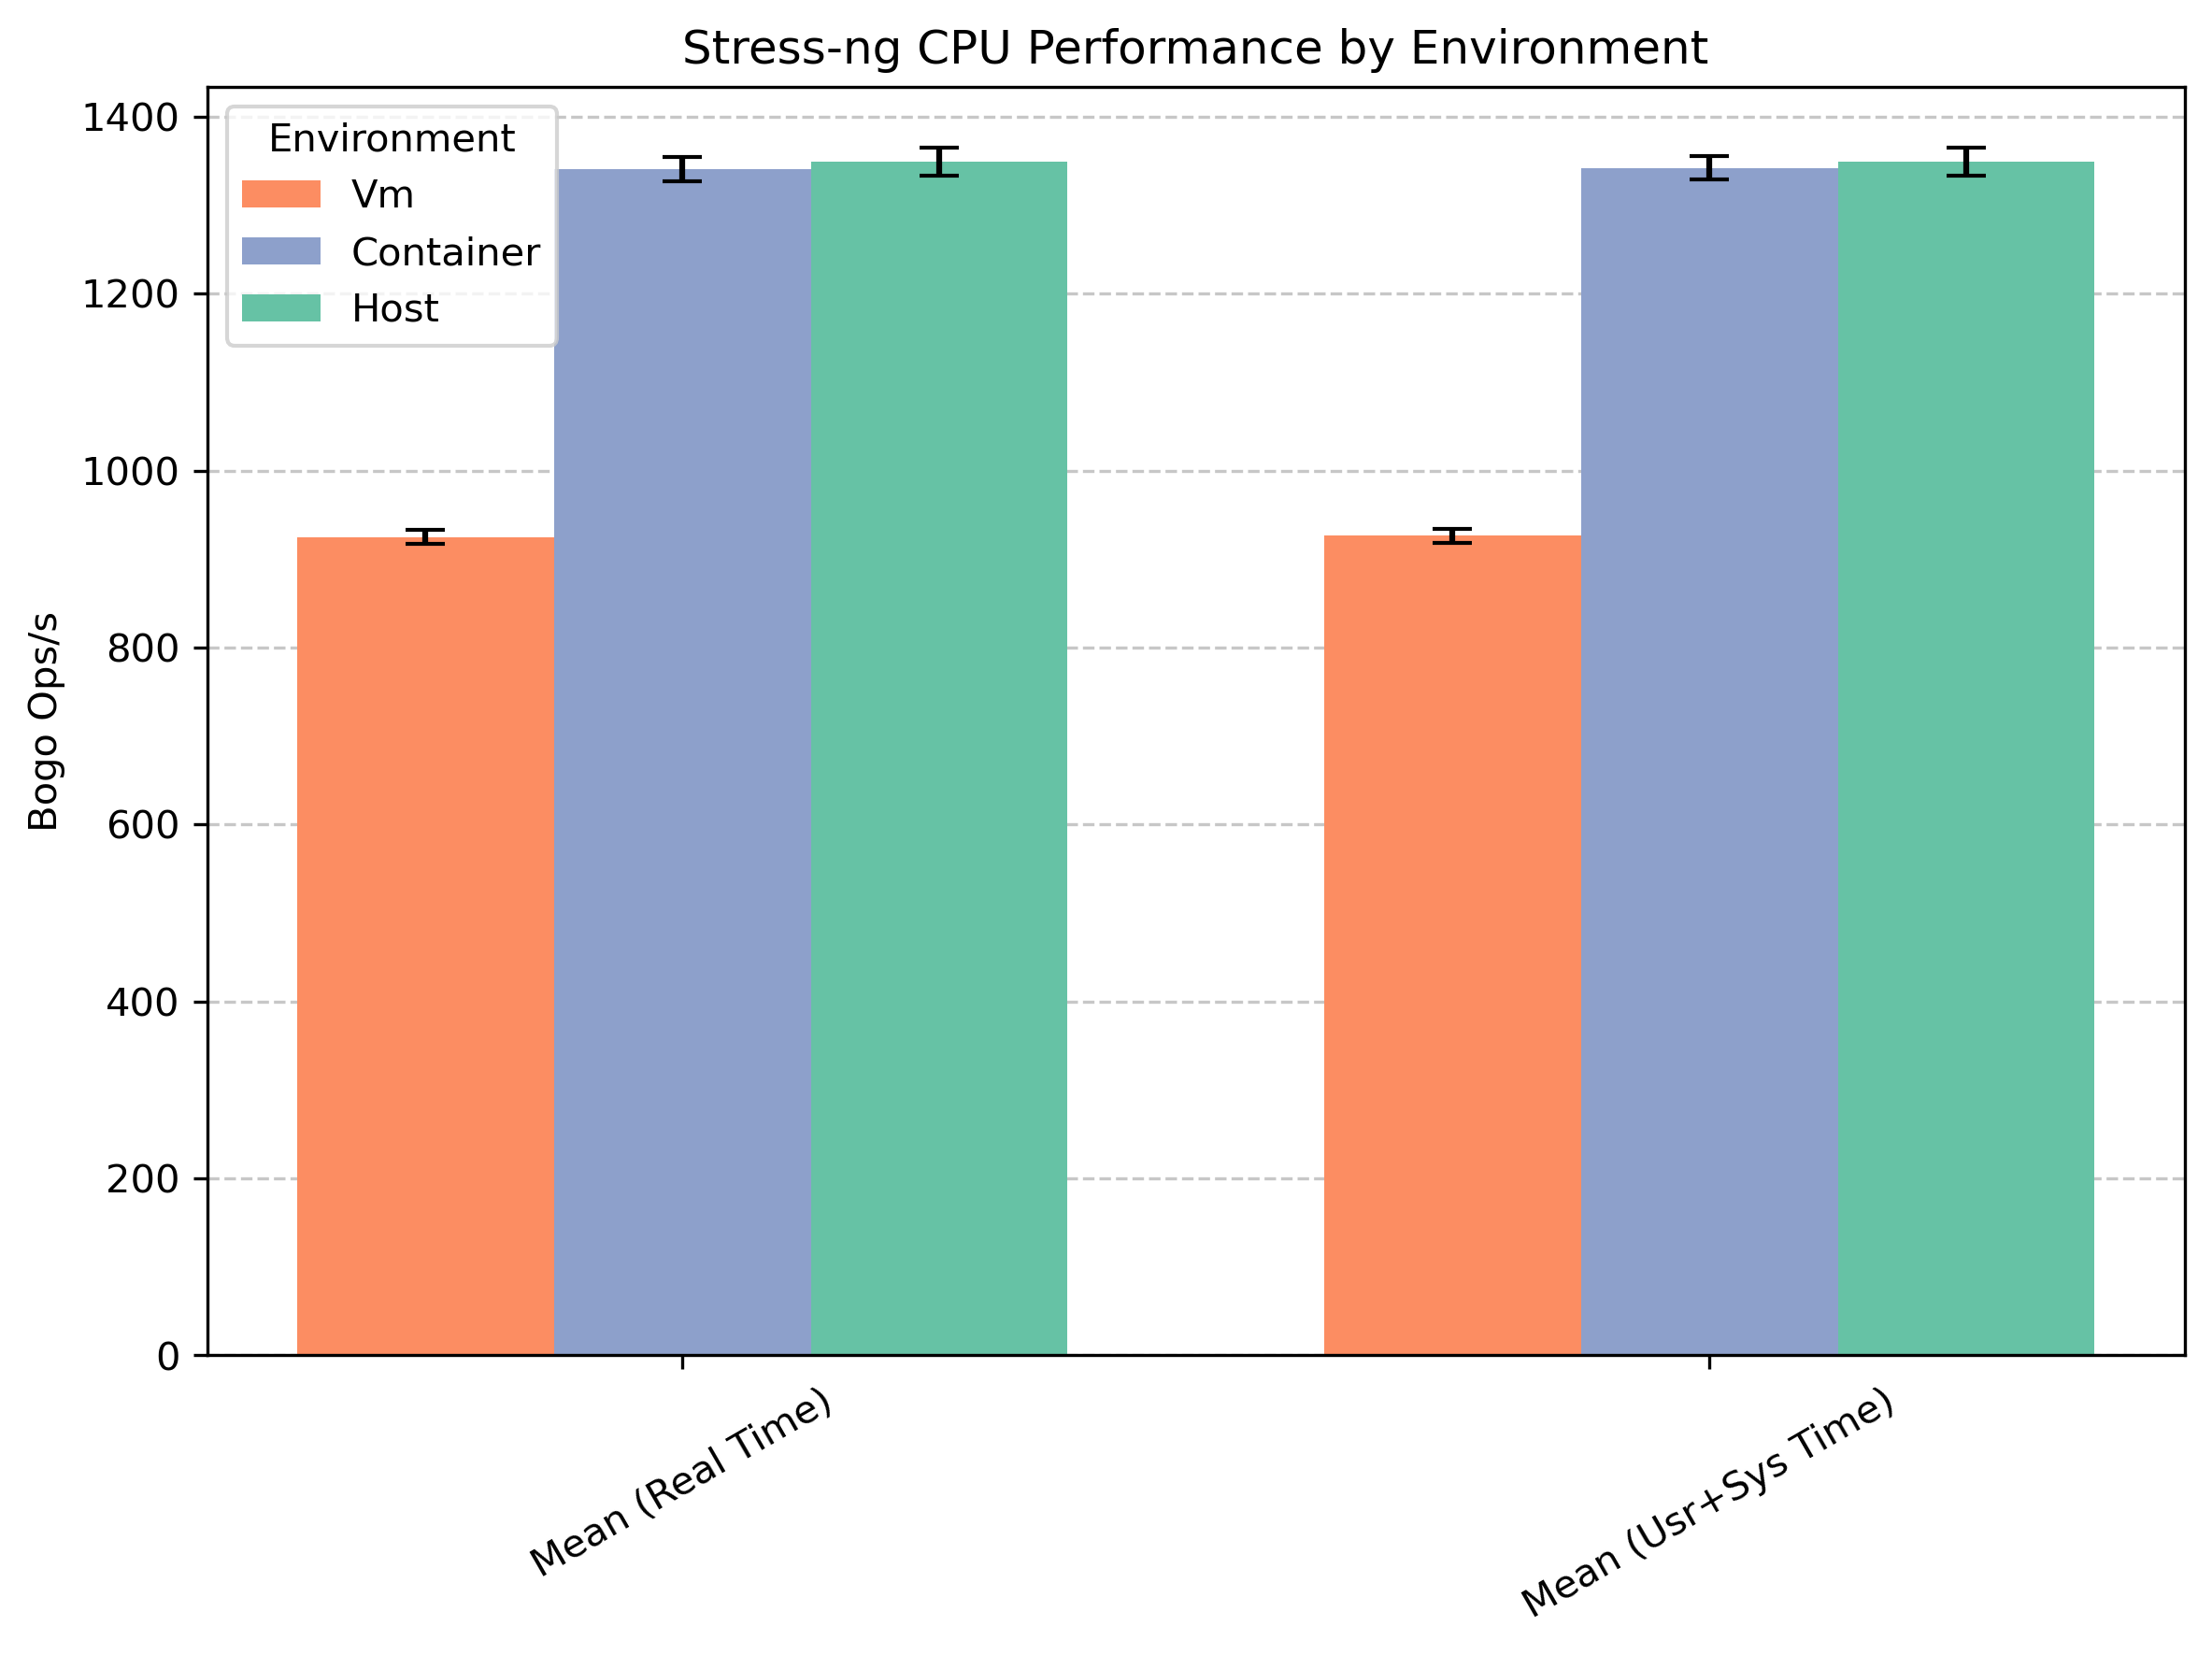
\includegraphics[width=0.6\textwidth]{stress_ng_cpu_performance.png}
  \end{figure}
  \begin{itemize}
    \item $\texttt{real} \approx \texttt{usr + sys}$: no significant waiting time
    \item VMs: fewer operations, higher CPU time per operation
  \end{itemize}
\end{frame}

\begin{frame}{Stress-ng: Memory}
  Repetitions: \textbf{5}
  \begin{figure}
    \centering
    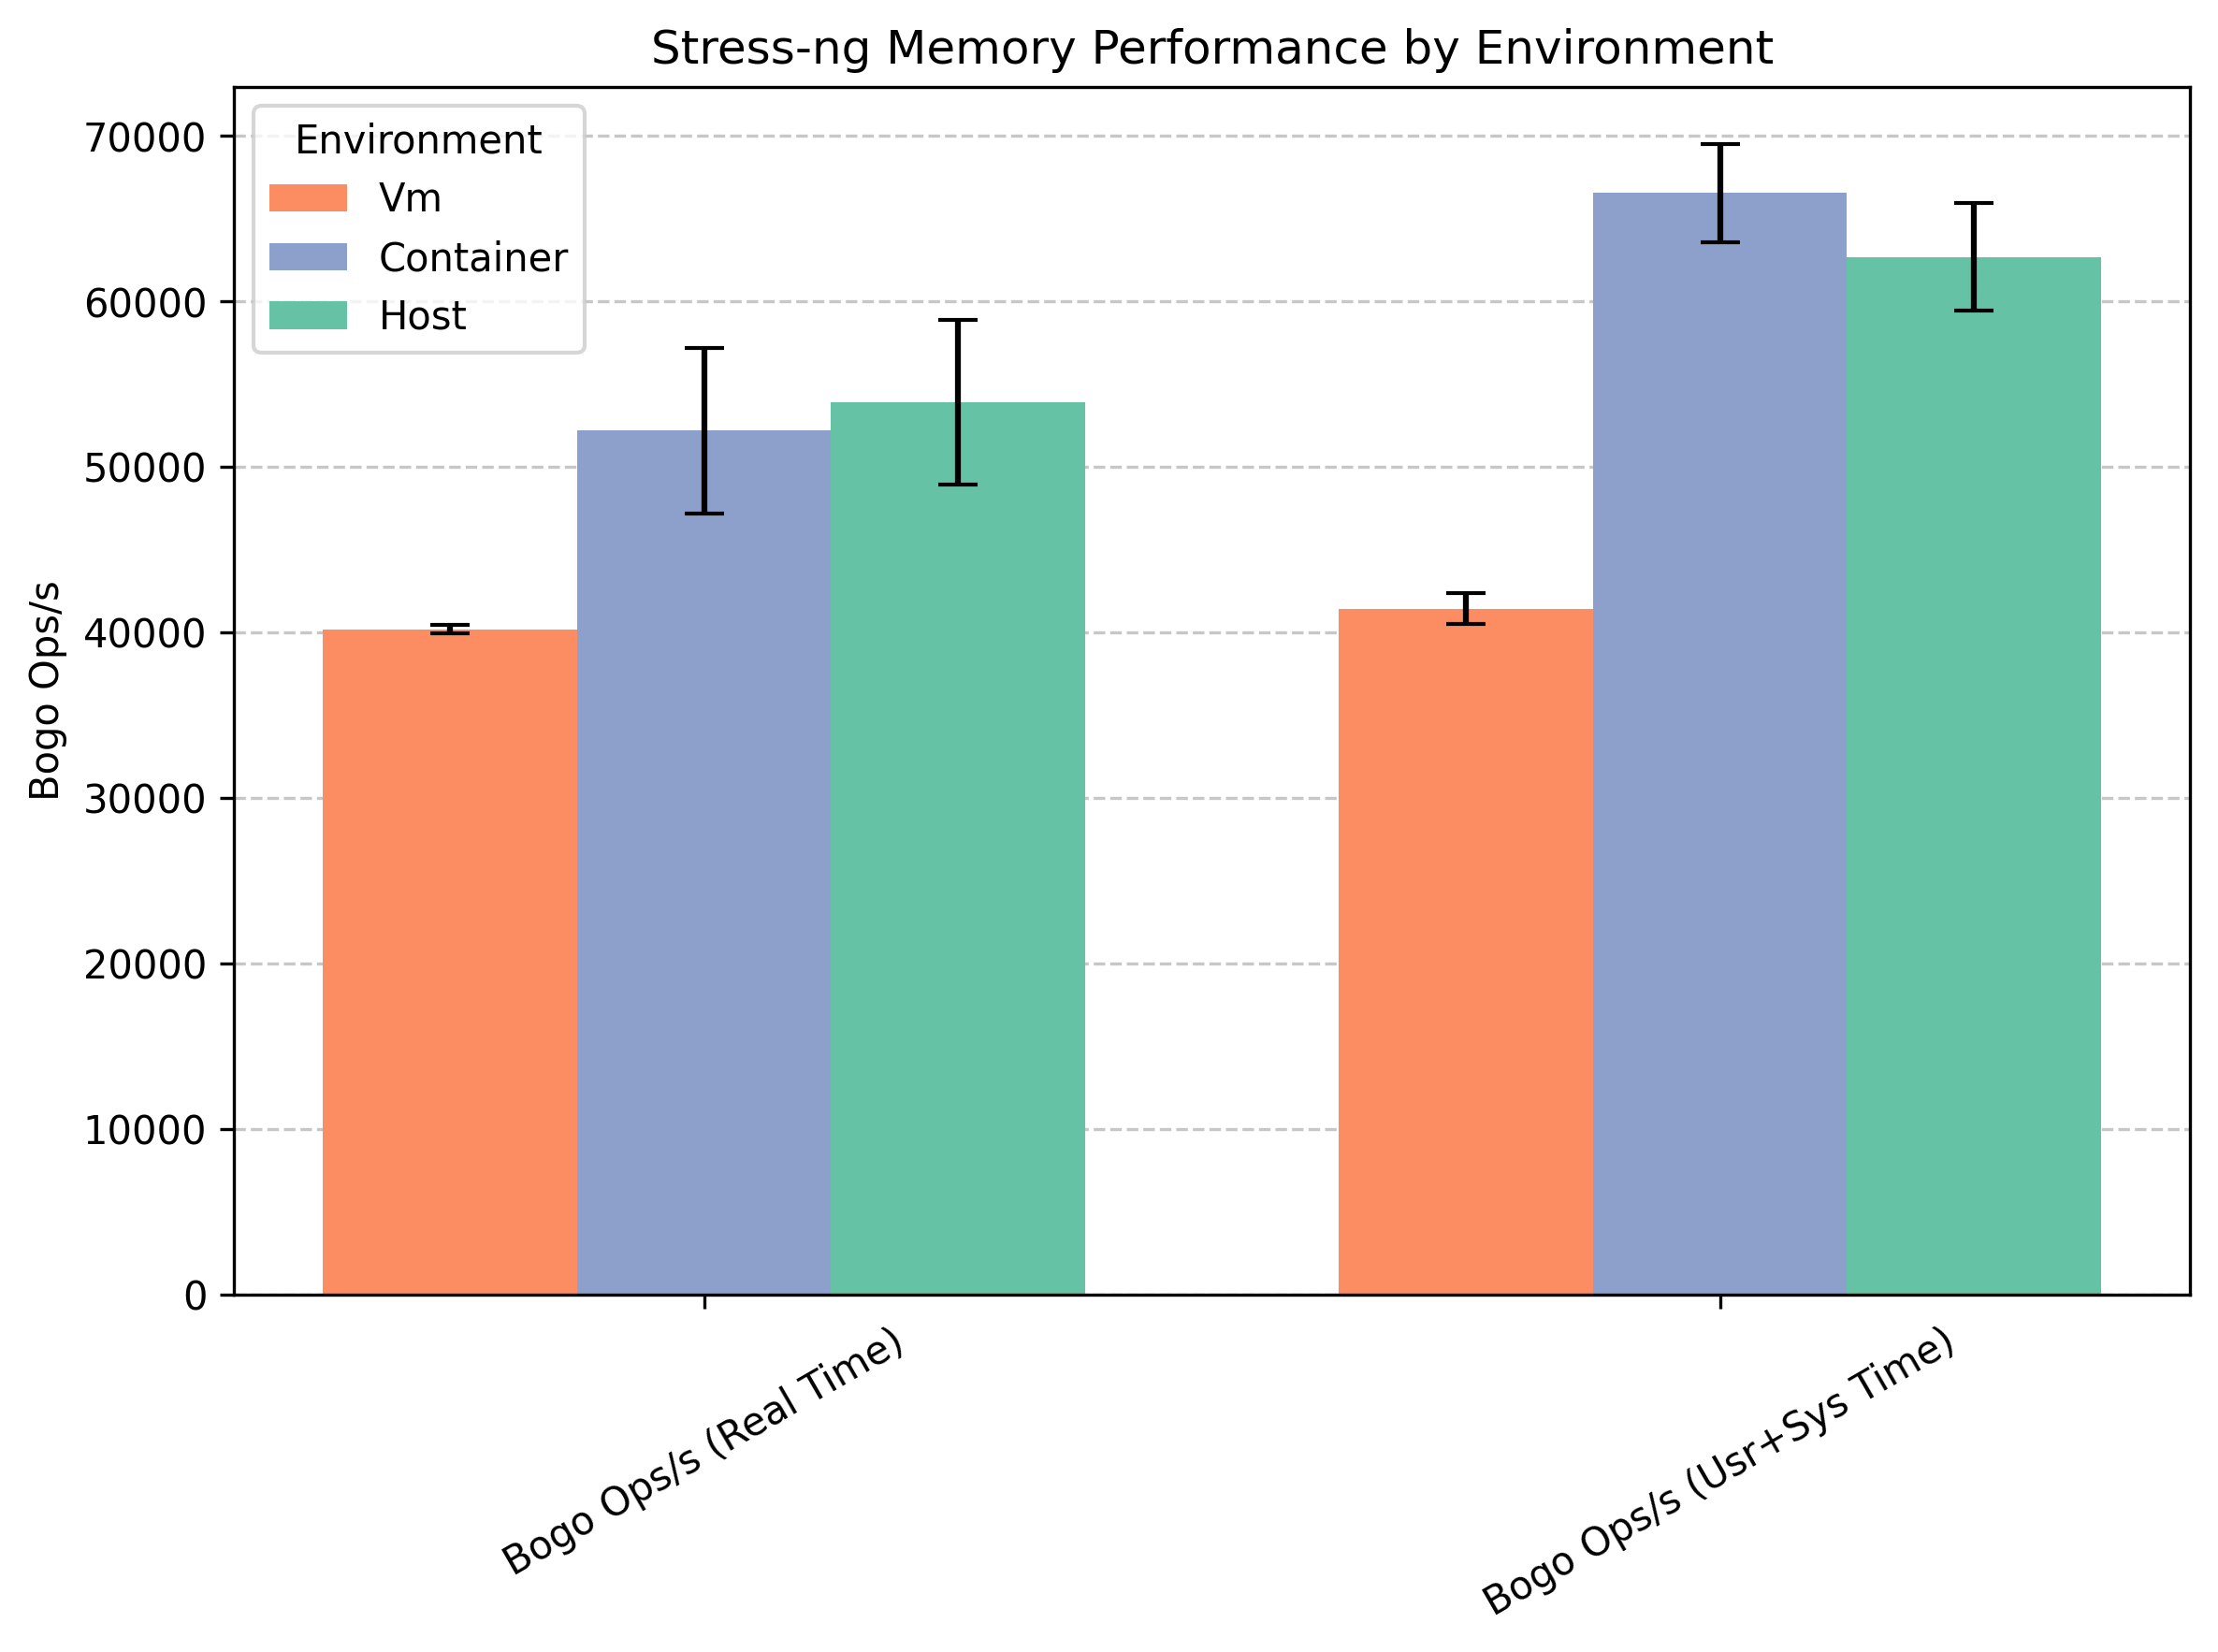
\includegraphics[width=0.6\textwidth]{stress_ng_memory_performance.png}
  \end{figure}
  \begin{itemize}
    \item Containers and Host: $\texttt{real} > \texttt{usr + sys}$ → some waiting time
    \item VMs: $\texttt{real} \approx \texttt{usr + sys}$ → less waiting, but still higher CPU time per operation
  \end{itemize}
\end{frame}


\begin{frame}{Sysbench}
  Number of repetition: \textbf{5}
  \begin{table}[htbp]
    \centering
    \footnotesize
    \begin{tabular}{lccc}
    \toprule
    \textbf{Benchmark} & \textbf{VM} & \textbf{Container} & \textbf{Host} \\
    \midrule
    \textbf{CPU} & & & \\
    Events/s & $453.97 \pm 1.28$ & $459.74 \pm 2.54$ & $452.38 \pm 6.76$ \\
    Latency sum (ms) & $9998.15 \pm 0.70$ & $9999.55 \pm 0.51$ & $9999.56 \pm 0.72$ \\
    \midrule
    \textbf{Memory} & & & \\
    Throughput (Gib/s) & $3.88 \pm 0.02$ & $\mathbf{5.51 \pm 0.09}$ & $5.19 \pm 0.08$ \\
    Latency sum (ms) & $1066.09 \pm 8.01$ & $\mathbf{839.99 \pm 14.63}$ & $895.79 \pm 18.40$ \\
    \bottomrule
    \end{tabular}
\end{table}
\end{frame}

\begin{frame}{IOZone: write local}
  \begin{figure}
    \centering
    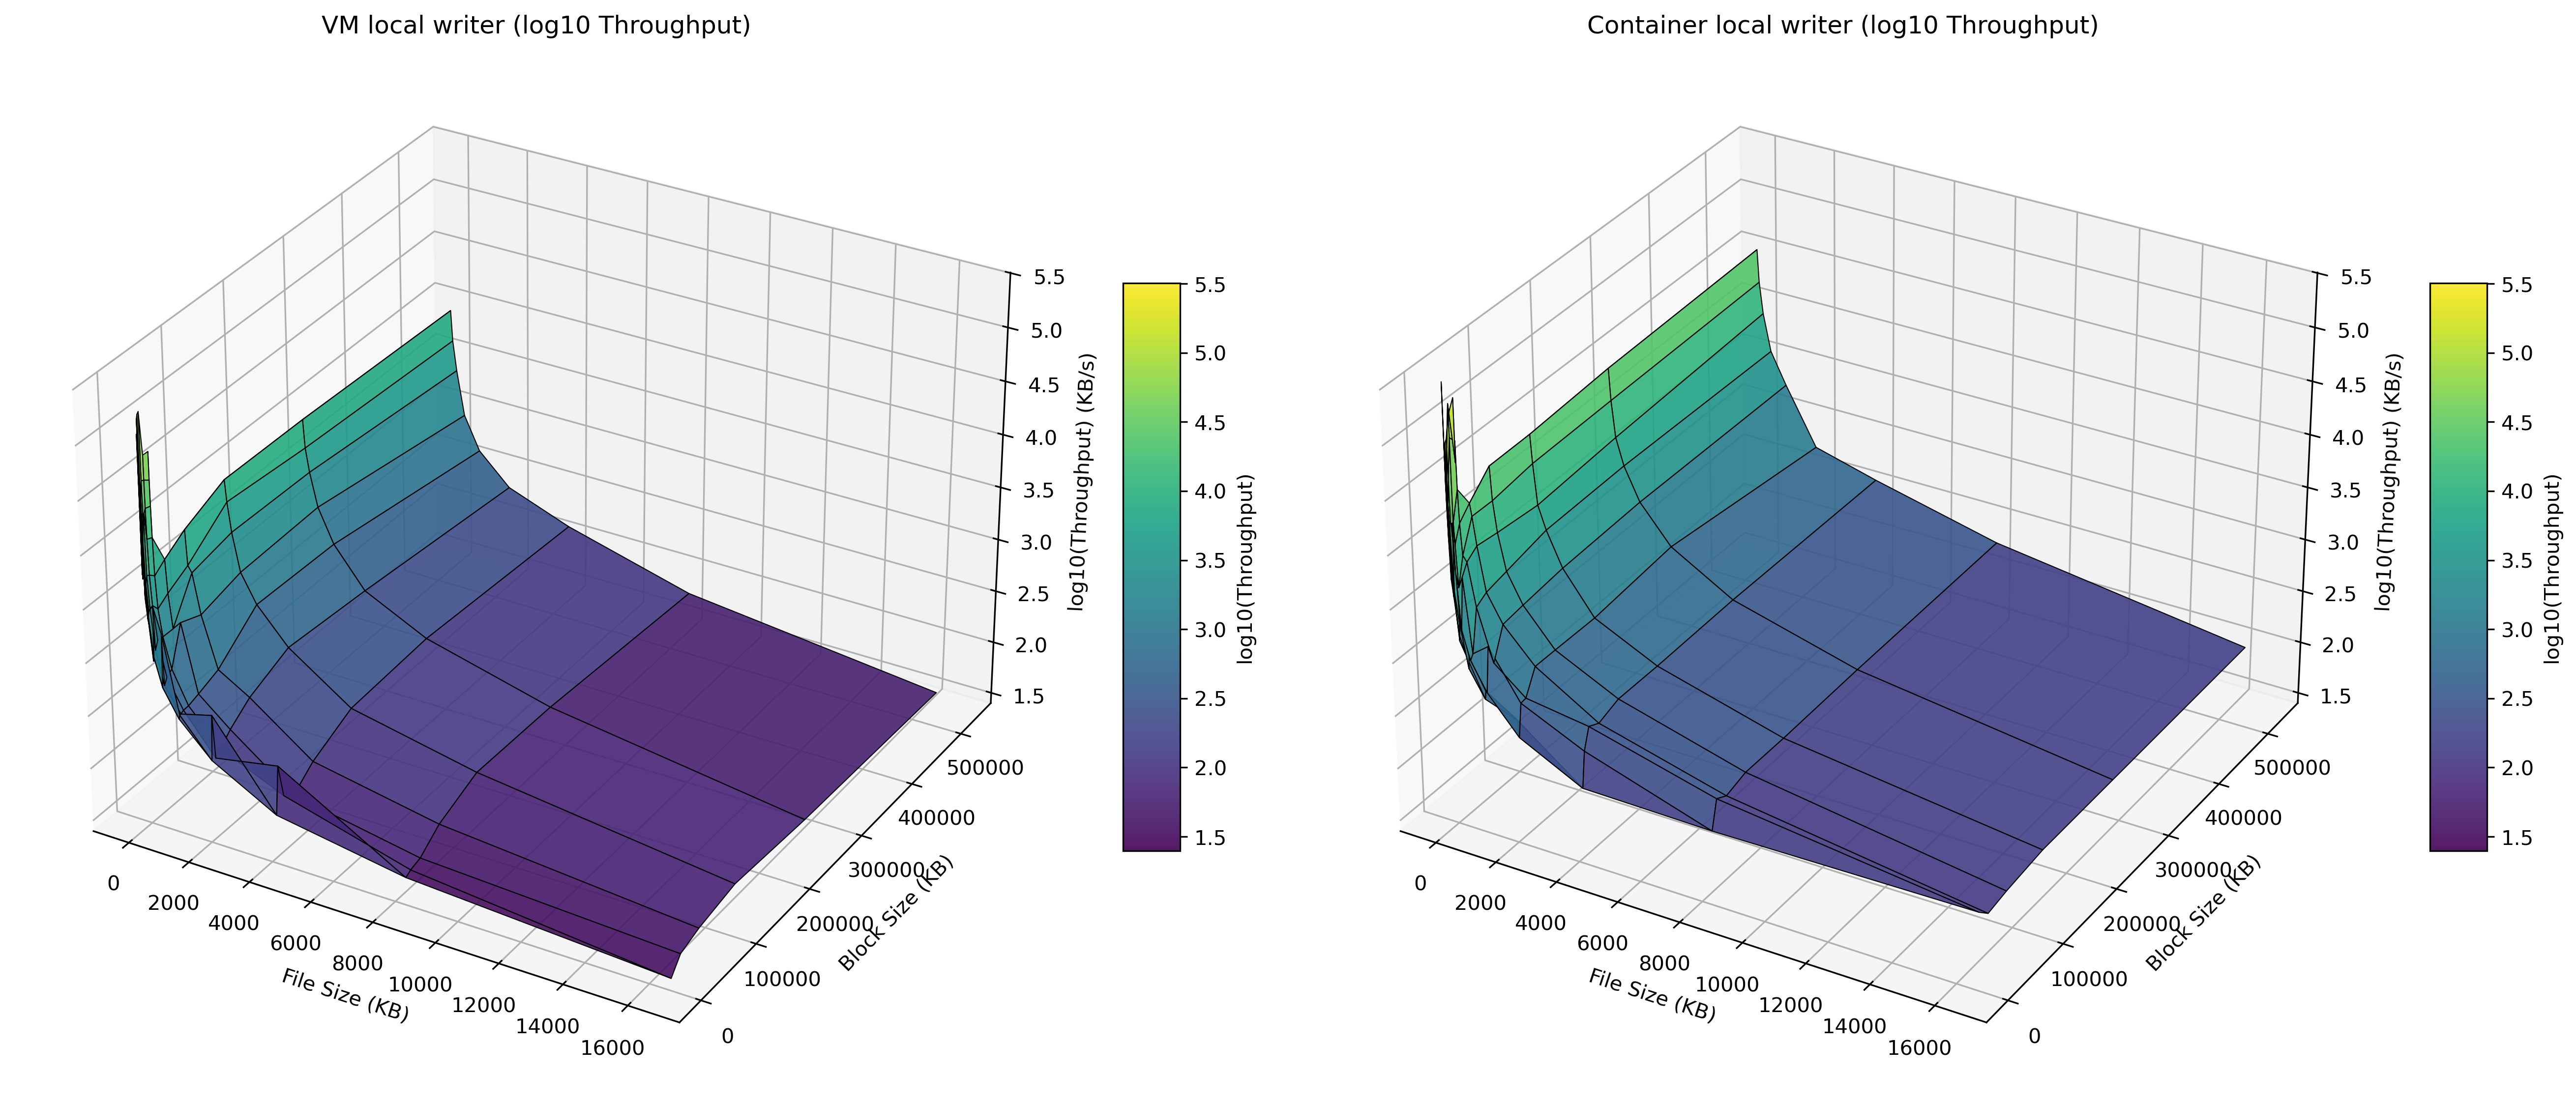
\includegraphics[width=\textwidth]{VM local writer_Container local writer_log_surfaces.png}
  \end{figure}
\end{frame}

\begin{frame}{IOZone: write shared}
  \begin{figure}
    \centering
    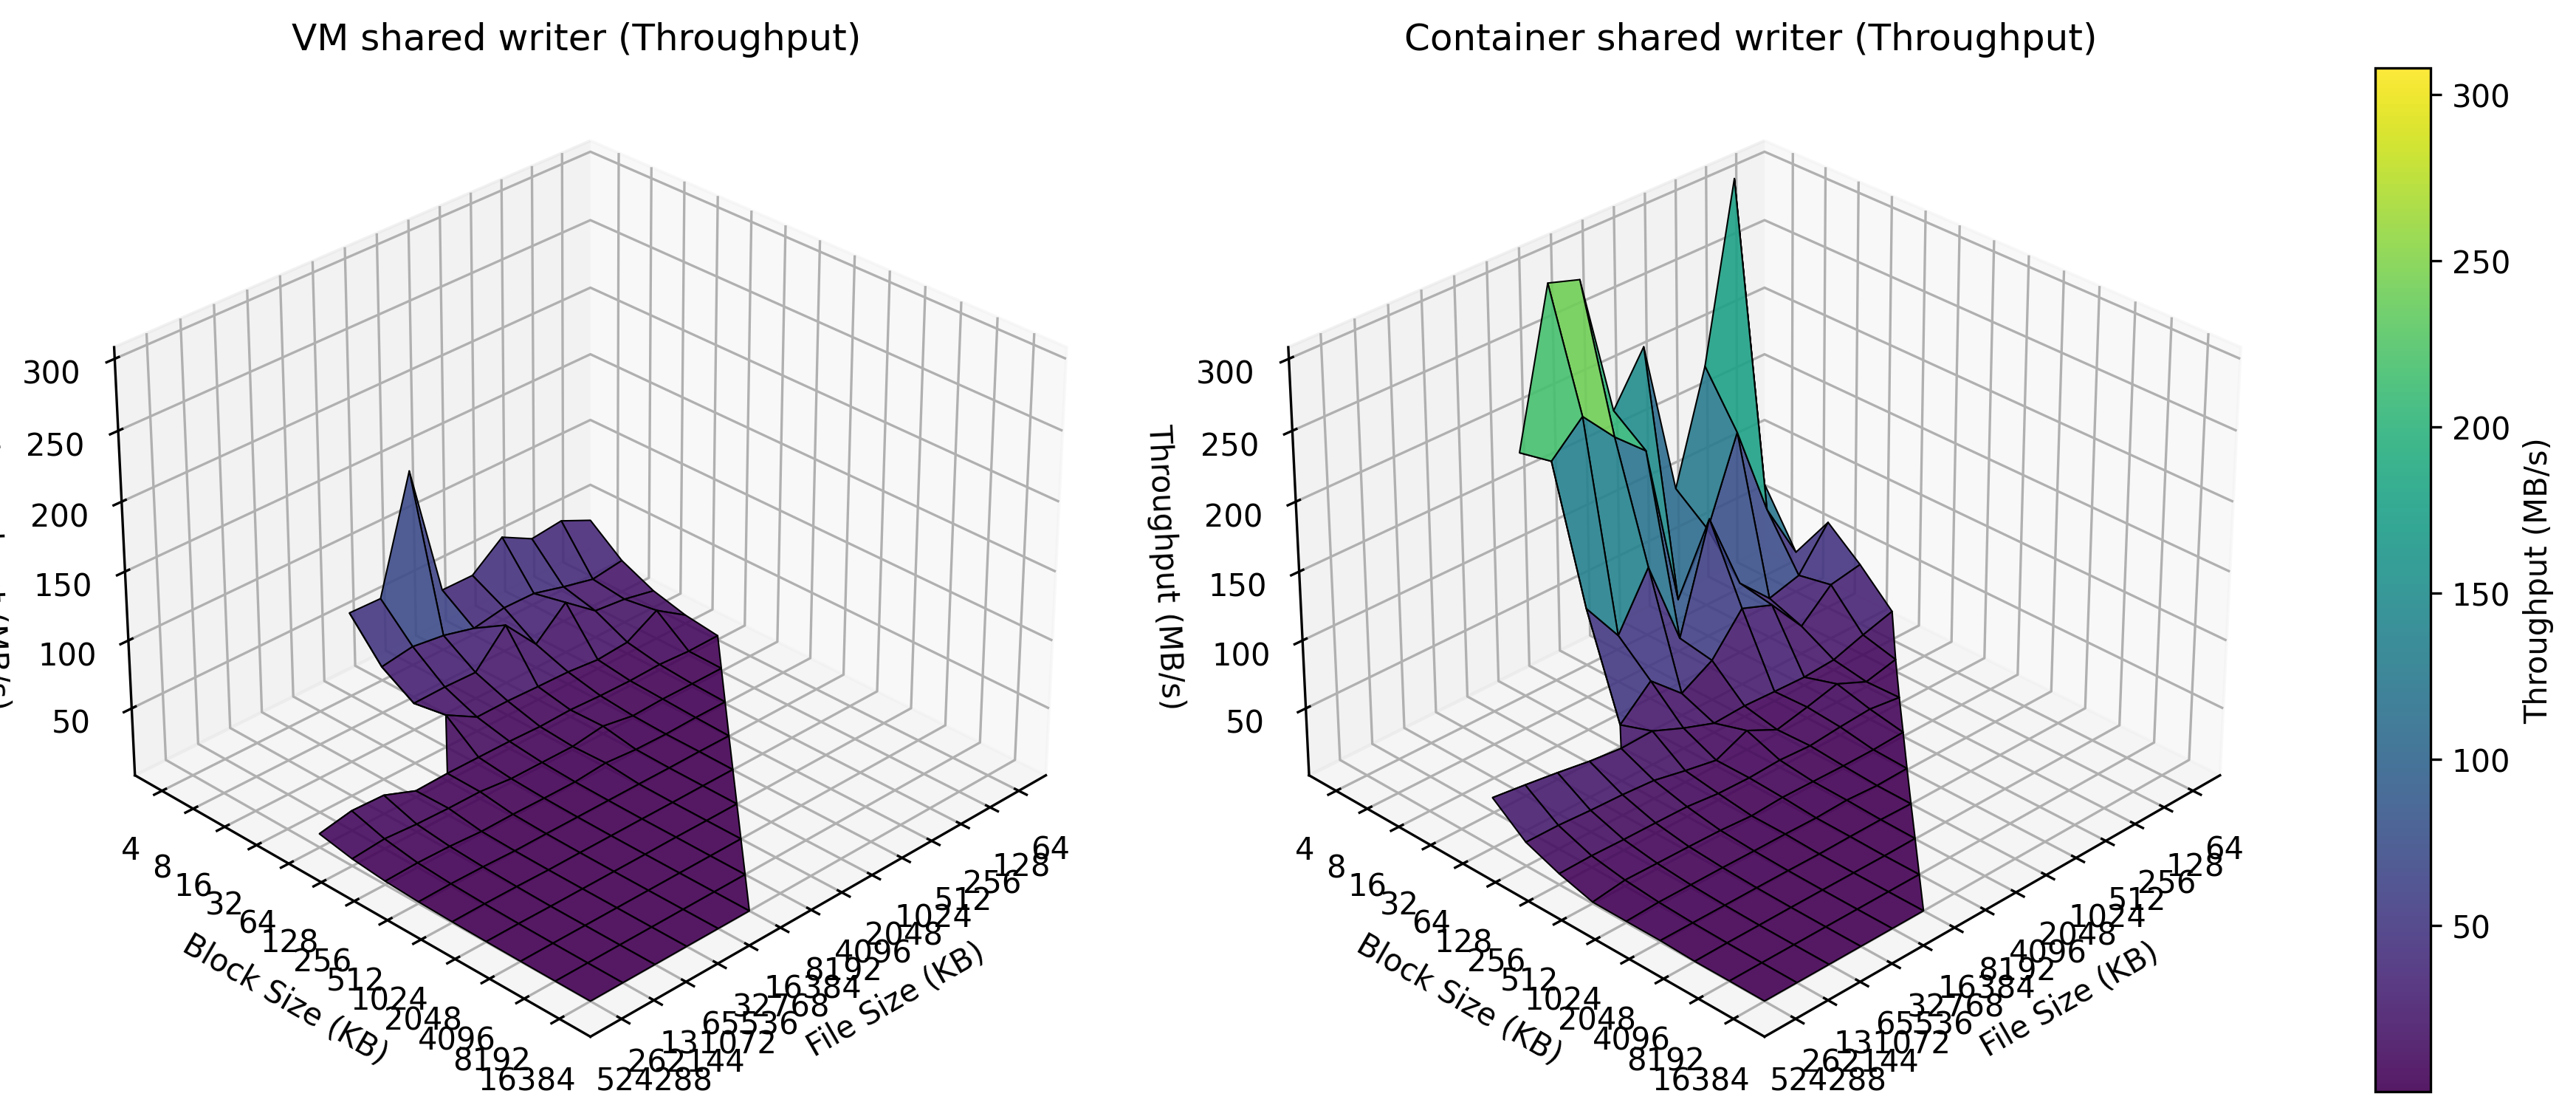
\includegraphics[width=\textwidth]{VM shared writer_Container shared writer_log_surfaces.png}
  \end{figure}
\end{frame}

\begin{frame}{IOZone: writing comparison}
  \begin{figure}
    \centering
    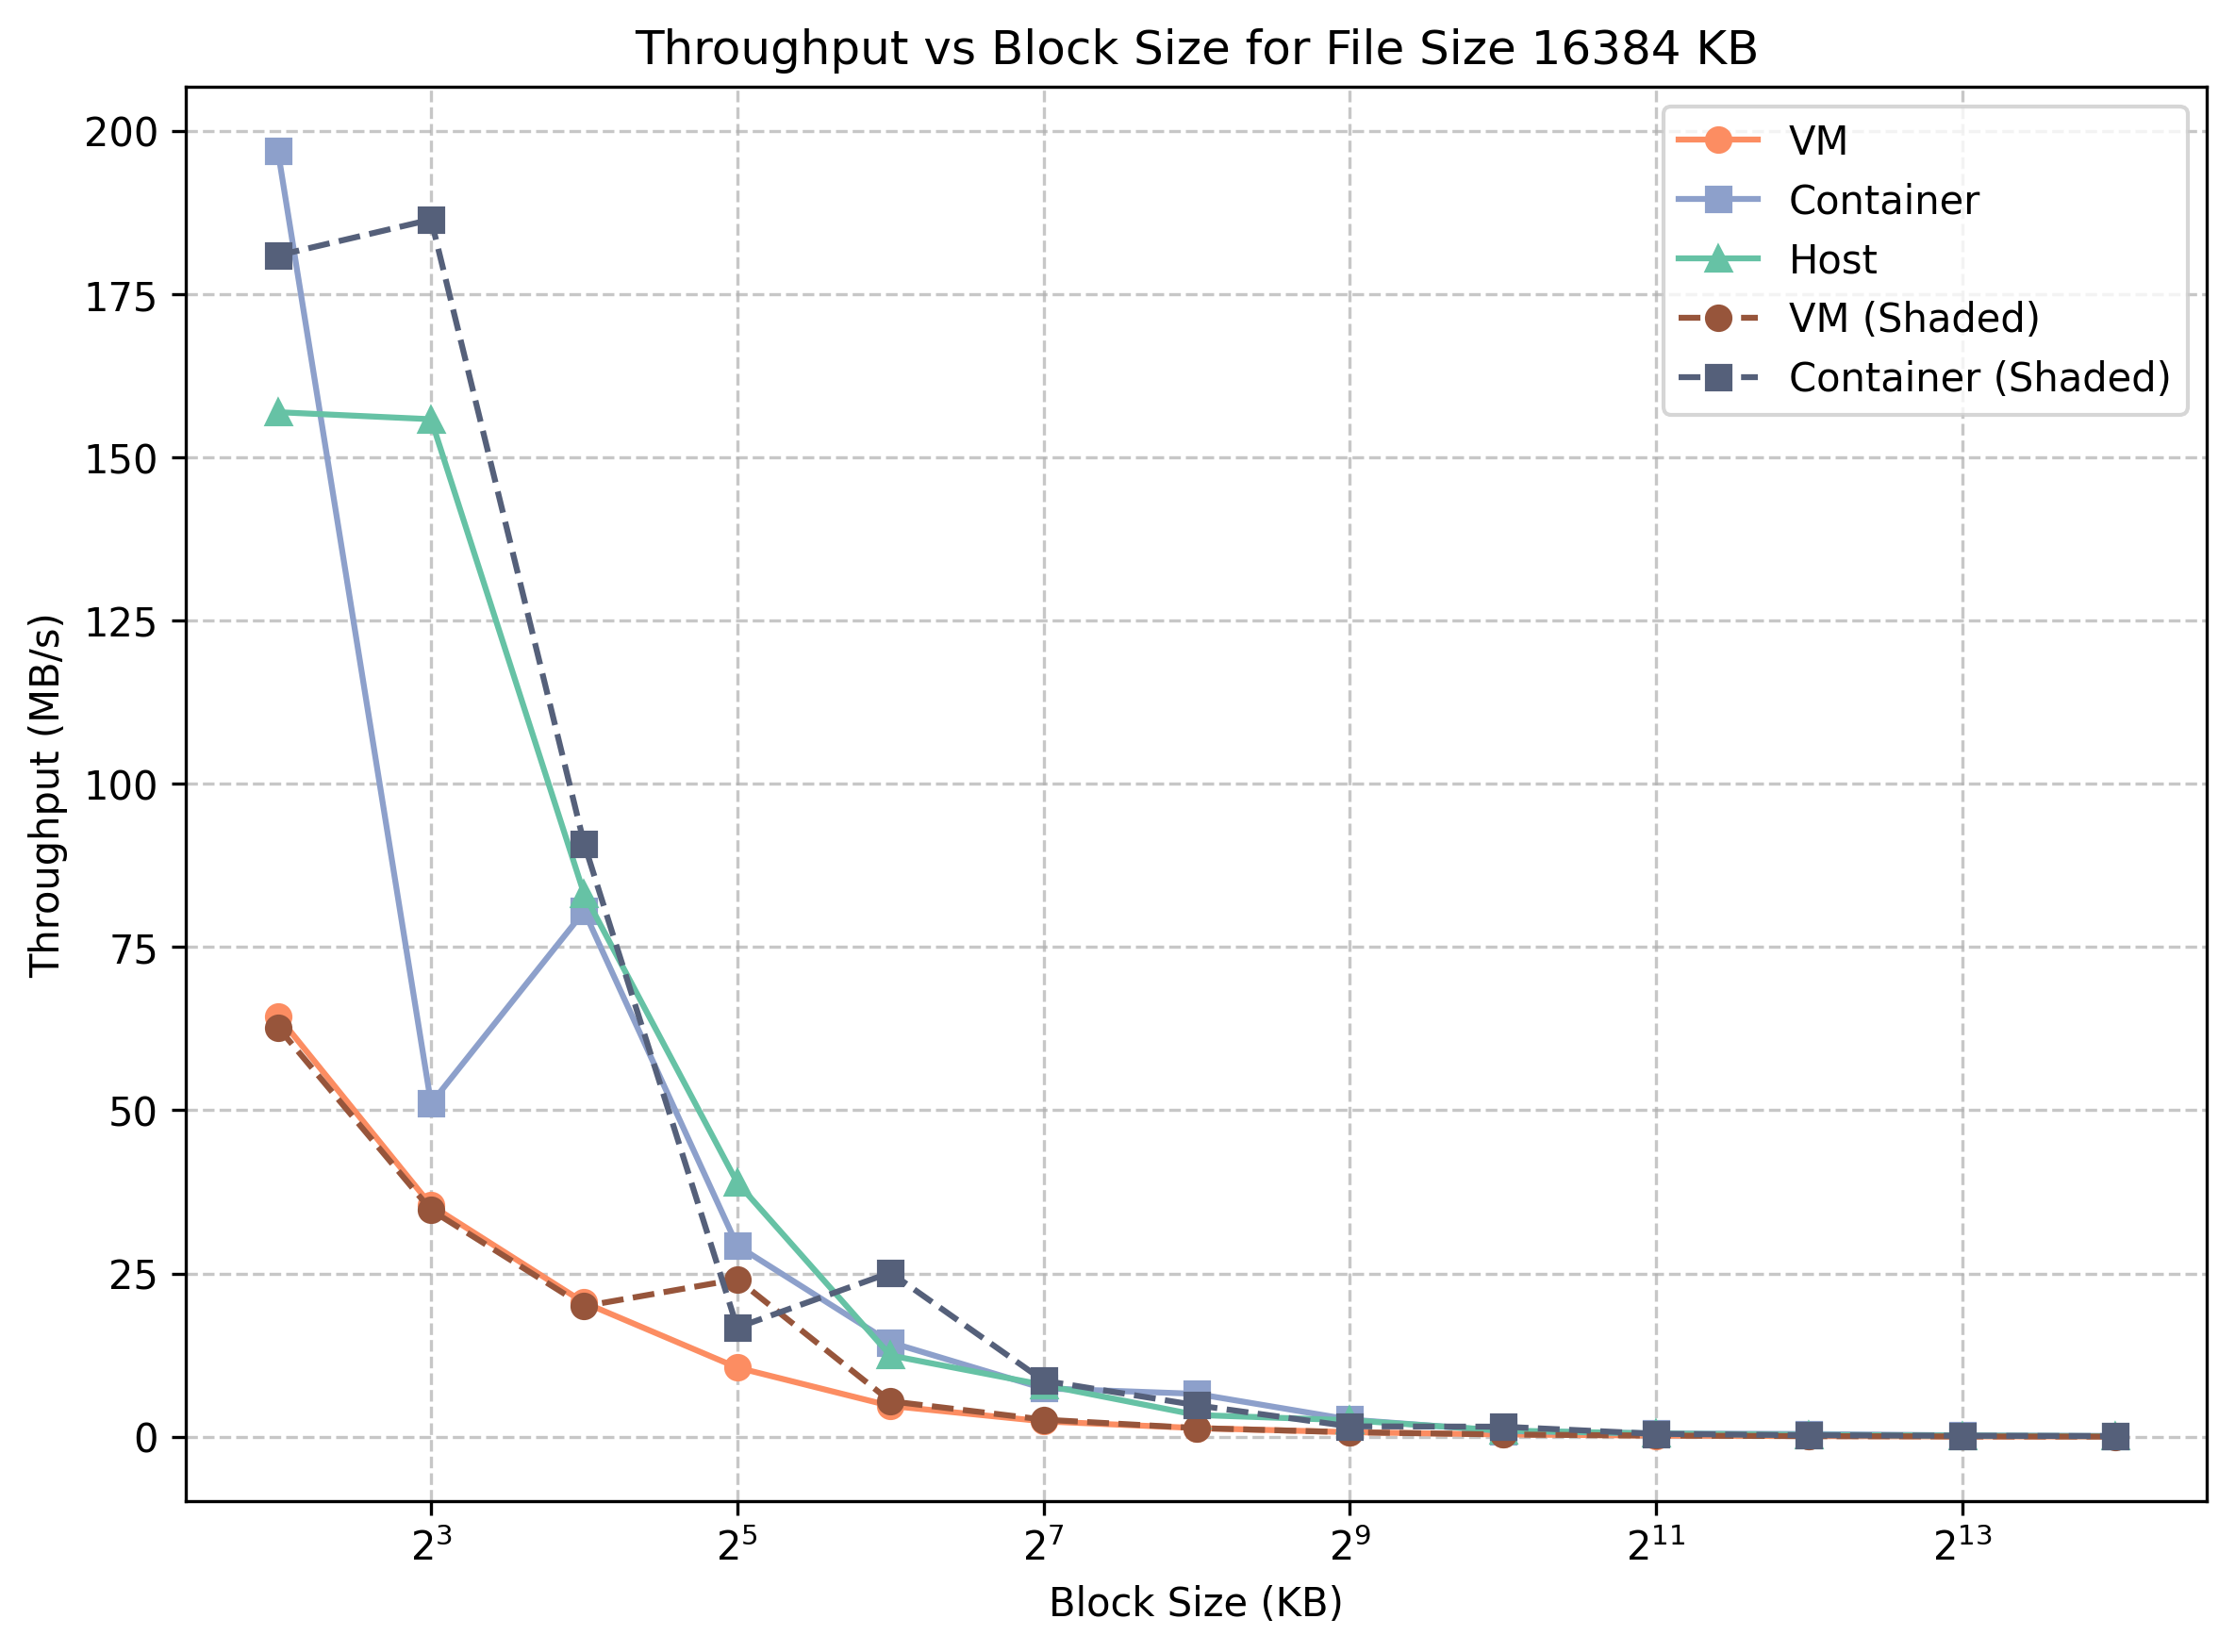
\includegraphics[width=0.7\textwidth]{writer_filesize_16384.png}
  \end{figure}
\end{frame}

\begin{frame}[fragile]{Iperf}
\begin{figure}
  \centering
  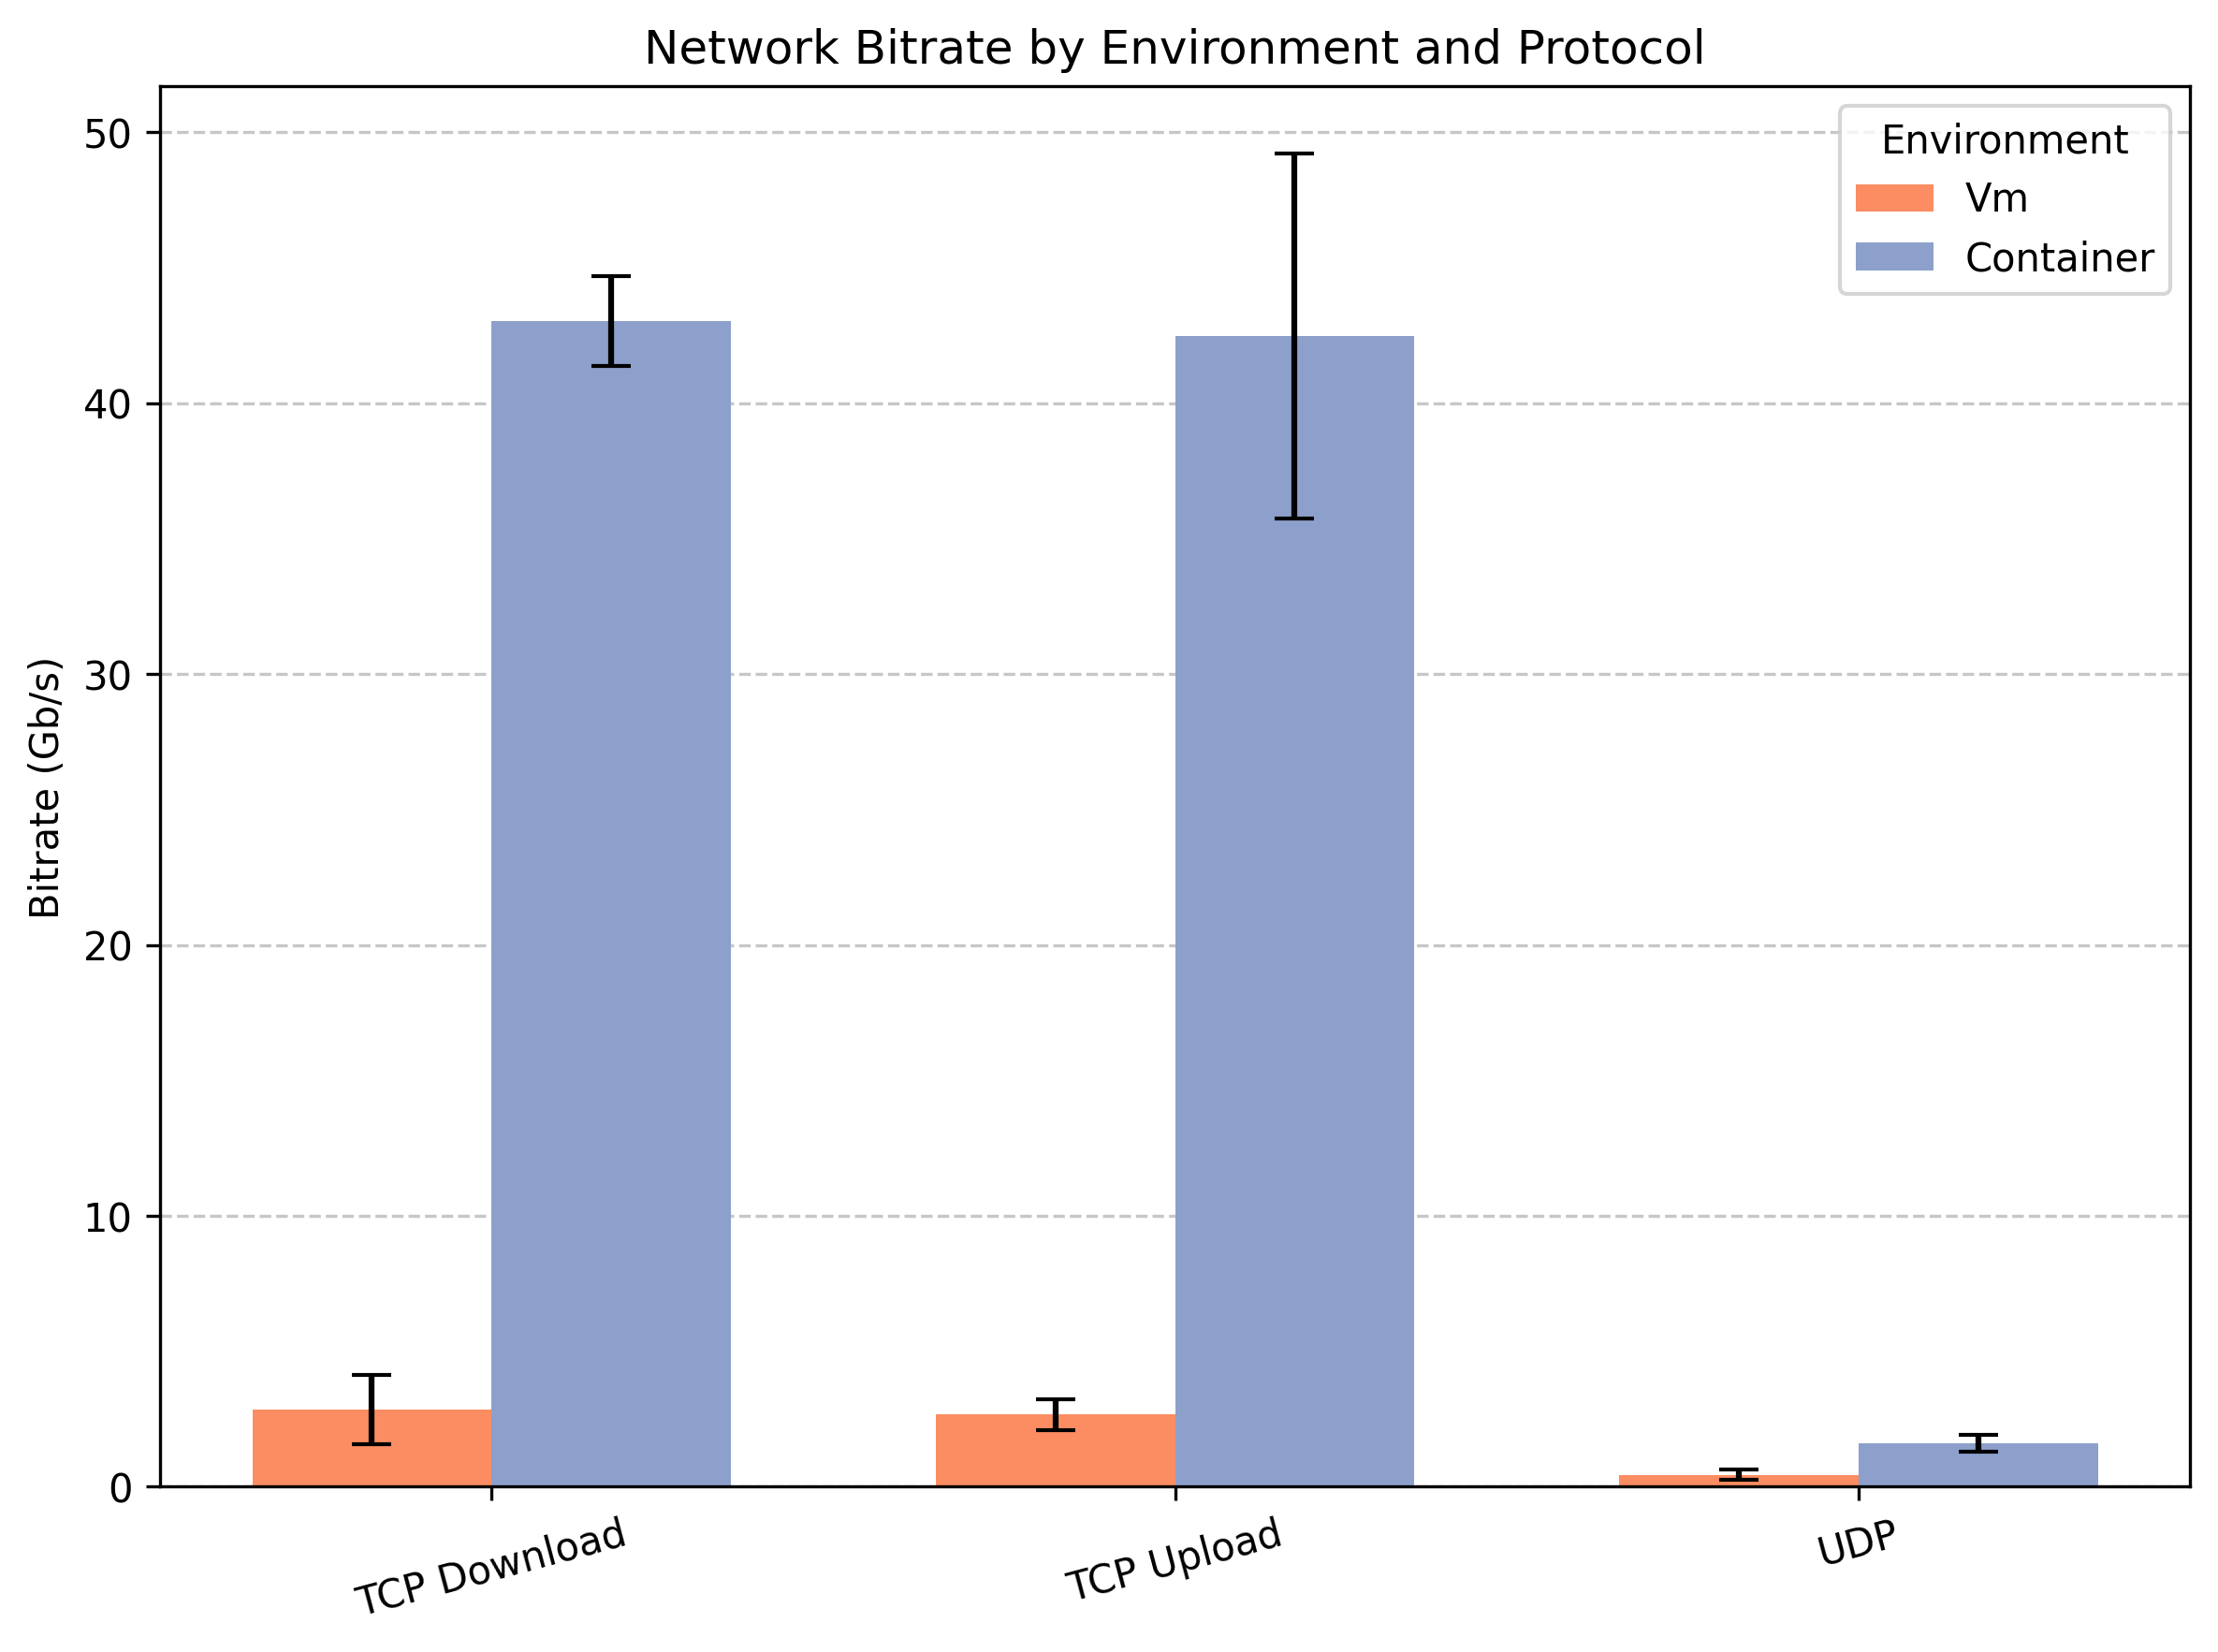
\includegraphics[width=0.7\textwidth]{network_bitrate_performance.png}
  % You can add a caption here if needed: \caption{Network Bitrate Performance}
\end{figure}
\end{frame}

\section{Conclusion}

\begin{frame}{Conclusion}
  \textbf{Docker Cluster}
  \begin{itemize}
    \item Easier to configure (shared kernel and lightweight setup)
    \item Near-native or better performance in CPU and memory benchmarks
    \item More scalable
  \end{itemize}
  \textbf{VirtualBox Cluster}
  \begin{itemize}
    \item More time-consuming to configure (multiple full OS instances)
    \item Higher overhead due to full hardware virtualization
    \item Lower memory bandwidth and network bitrate observed
  \end{itemize}
\end{frame}

{\setbeamercolor{palette primary}{fg=white, bg=bluscuro}
\begin{frame}[standout]
\thispagestyle{empty}
  {\LARGE Thank You!}
\end{frame}
}



\end{document}
